% コンパイル: lualatex paper_ja.tex
\documentclass[10pt,twocolumn]{ltjsarticle}
\usepackage{luatexja-fontspec}
\usepackage[a4paper,margin=18mm]{geometry}
\usepackage{graphicx}
\usepackage{amsmath}
\usepackage{booktabs}
\usepackage{enumitem}
\usepackage[hidelinks]{hyperref}

\setlength{\columnsep}{6mm}

\begin{document}

\twocolumn[{%
  \begin{center}
    {\LARGE\bfseries 個人制作キャラクターの画像生成LoRAファインチューニング}\\
    \vspace{0.6em}
    {\large ——消費者向けGPUによる実験的検討——}\\
    \vspace{1.2em}
    {\large Masato Suzuki (Masafy)}\\
    \vspace{0.4em}
    {2026年5月22日}
  \end{center}
  \vspace{1.0em}
  {\centering\textbf{要 旨}\par}
  \vspace{0.4em}
  \begingroup\small
  \noindent 本報告では、著者が個人制作したオリジナルキャラクター「マサフィー」（LINEスタンプとして公開済みのレッサーパンダキャラクター）の新規イラストを生成することを目的として、Stable Diffusion 1.5 に対する LoRA（Low-Rank Adaptation）ファインチューニングを行った。学習にはクラウドの有料計算資源を用いず、消費者向けGPUである NVIDIA GeForce RTX 3060（VRAM 12GB）を搭載した自宅PCのみを使用した。既存スタンプ16点から品質基準で13点を選定して学習データとし、(1) 初回学習による実現可能性検証、(2) ベースモデル・学習率・LoRA次元を変化させた6条件の比較実験、(3) エポック数10〜60の追加学習による過学習点の特定、の3段階の実験を実施した。その結果、(a) ベースモデルの選択が出力品質に最も大きく影響し、イラスト指向モデルを用いることで背景・画風の問題が解消されること、(b) 学習エポック数は約30で性能が頭打ちとなり、それ以降は改善せず軽度の過学習傾向を示すこと、(c) 出力品質の上限は学習画像枚数によって規定されること、を明らかにした。本実験を通じて、消費者向けGPU 1台で実用的なキャラクターLoRAの作成が完結可能であることを確認した。

  \par\medskip
  \noindent\textbf{キーワード:}\ 画像生成, Stable Diffusion, LoRA, ファインチューニング, キャラクター生成, 消費者向けGPU
  \endgroup
  \vspace{2.2em}
}]

\section{はじめに}
近年、テキストから画像を生成する拡散モデル（diffusion model）が広く普及し、Stable Diffusion をはじめとするオープンなモデルが個人でも利用可能となった。一方で、特定のオリジナルキャラクターを一貫した見た目で生成するには、汎用モデルそのままでは不十分であり、追加学習が必要となる。

LoRA（Low-Rank Adaptation）は、巨大なモデル全体を再学習する代わりに、低ランクの差分行列のみを学習する手法であり、少ない計算資源と少数の学習画像で特定の概念をモデルに追加できる。これにより、個人が所有するキャラクターの追加学習が現実的になっている。

本研究の動機は実用的である。著者は「マサフィー」というレッサーパンダのオリジナルキャラクターを制作し、LINEスタンプとして公開している（全16種）。このキャラクターの新しいポーズや場面のイラストを、追加で描かずに生成したいというのが出発点である。

検討にあたり、当初は有料クラウド計算環境（Google Colab Pro+ 等）の利用も候補としたが、本研究では自宅にある消費者向けGPU 1台のみで完結できるかを検証することとした。具体的な問いは以下の3点である。
\begin{itemize}[leftmargin=2.2em,topsep=2pt,itemsep=1pt]
  \item[\textbf{Q1.}] 13枚程度の少数画像で、キャラクターの同一性を保ったまま新規ポーズを生成できるか。
  \item[\textbf{Q2.}] 出力品質を左右する要因は何か（ベースモデル・学習率・LoRA次元・エポック数）。
  \item[\textbf{Q3.}] 学習エポック数を増やせば品質は向上し続けるのか。
\end{itemize}

\section{関連手法}
Stable Diffusion は潜在拡散モデル（latent diffusion model）であり、本研究では広く普及している SD 1.5 系列を対象とした。LoRA はモデルの重み行列 $W$ に対し低ランク差分 $\Delta W = BA$ のみを学習する手法で、学習対象パラメータを大幅に削減する。学習には kohya-ss 氏による \texttt{sd-scripts}（LoRA学習の事実上の標準実装の一つ）を用いた。

\section{手法}
\subsection{計算環境}
計算環境を表\ref{tab:env}に示す。OS 標準の Python 3.14 では学習ツール群が依存解決できなかったため、軽量Python管理ツール \texttt{uv} を用いて Python 3.11 環境を分離構築した。これは最新のディストリビューションで学習環境を構築する際の実務的な留意点である。

\begin{table*}[t]\centering\small
\caption{計算環境}
\label{tab:env}
\begin{tabular}{ll}
\toprule
項目 & 内容 \\
\midrule
GPU & NVIDIA GeForce RTX 3060（VRAM 12GB, Ampere, compute capability 8.6） \\
CPU / RAM & 20論理コア / 30GB \\
OS & Ubuntu 26.04 LTS \\
学習フレームワーク & kohya-ss/sd-scripts, PyTorch 2.5.1 + CUDA 12.4 \\
Python環境 & システムPython（3.14）が非対応のため \texttt{uv} で Python 3.11 を別途導入 \\
\bottomrule
\end{tabular}
\end{table*}

\subsection{学習データ}
学習データは、著者制作のLINEスタンプ「マサフィー」全16種を出発点とした。図\ref{fig:data}に示すとおり、キャラクターはレッサーパンダをモチーフとし、ゴーグル・王冠柄のバンダナ・縞模様の尾といった一貫した特徴を持つ。16種のうち、解像度が著しく低い画像1点、画風が異なるラフスケッチ調の画像2点を除外し、\textbf{13点}を学習に用いた。採用画像はすべて 1000$\times$1000\,px・RGB である。

\begin{figure*}[t]\centering

\includegraphics[width=0.95\textwidth]{figures/fig1_trainingdata.png}
\caption{学習に用いたマサフィースタンプ13点。}
\label{fig:data}
\end{figure*}

\subsection{キャプション設計}
各画像には学習時に参照されるキャプションを付与した。固有語 \texttt{masafee} をトリガーワードとして全画像の先頭に固定し、可変としたい属性（ポーズ・表情・背景・文字の有無）はキャプションに明記した。一方、キャラクター固有の不変要素（ゴーグル、バンダナ等）はあえて記述せず、トリガーワード自体に結びつくようにした。スタンプに焼き込まれた文字は、トリミング除去せず「文字を含む」旨をキャプションに記述して対処した。

\subsection{学習設定}
最適化手法は 8-bit AdamW、混合精度は bfloat16 とし、テキストエンコーダを含む LoRA を学習した。注意機構は PyTorch 標準の SDPA を用い、追加ライブラリへの依存を排した。

\section{実験}
\textbf{実験1（実現可能性検証）：} ベースモデルに標準 SD 1.5（\texttt{v1-5-pruned-emaonly}）、解像度512px、LoRA次元32／alpha16、学習率1e-4、16エポック（1040ステップ）で初回学習を行った。

\textbf{実験2（条件比較）：} ベースモデル\{標準SD1.5, Counterfeit-V3.0\}、学習率\{1e-4, 2e-4\}、LoRA次元\{16, 32\}を変化させた6条件を、解像度768px・各30エポックで学習・比較した。各保存点に対し学習データに無い5種の評価プロンプトで画像を生成し比較した。

\textbf{実験3（エポック数アブレーション）：} 実験2の最良条件を60エポックまで延長し、エポック30/40/50/60の出力を比較した。乱数シードは固定した。

\section{結果}
\subsection{実験1：初回学習は成功}
初回学習は RTX 3060 で約9分、VRAM使用量は約3GBであった。キャラクターの同一性は良好に再現され、学習データに無いポーズも生成できた（\textbf{Q1は肯定的に確認}）。一方、(i)「白背景」と指定しても背景が暗色化する、(ii) 元のフラットな画風に比べ陰影が強い、という2つの弱点が観察された。

\subsection{実験2：ベースモデルが最も影響する}
6条件の比較結果は明瞭であった（図\ref{fig:sweep}）。標準SD1.5ベースの3条件はいずれも背景が暗色化し陰影が強い一方、Counterfeitベースの3条件は背景が白く整い、フラットな塗りで元のスタンプ画風に近い出力となった。すなわち実験1の弱点は、学習率やLoRA次元の調整ではなく、\textbf{ベースモデルをイラスト指向のものに変更することで解消された}。\textbf{Q2に対し、検討した要因の中ではベースモデル選択が支配的であると結論する。}最良条件は Counterfeit + 学習率1e-4 + LoRA次元32（cf\_lr1\_d32）とした。

\begin{figure*}[t]\centering
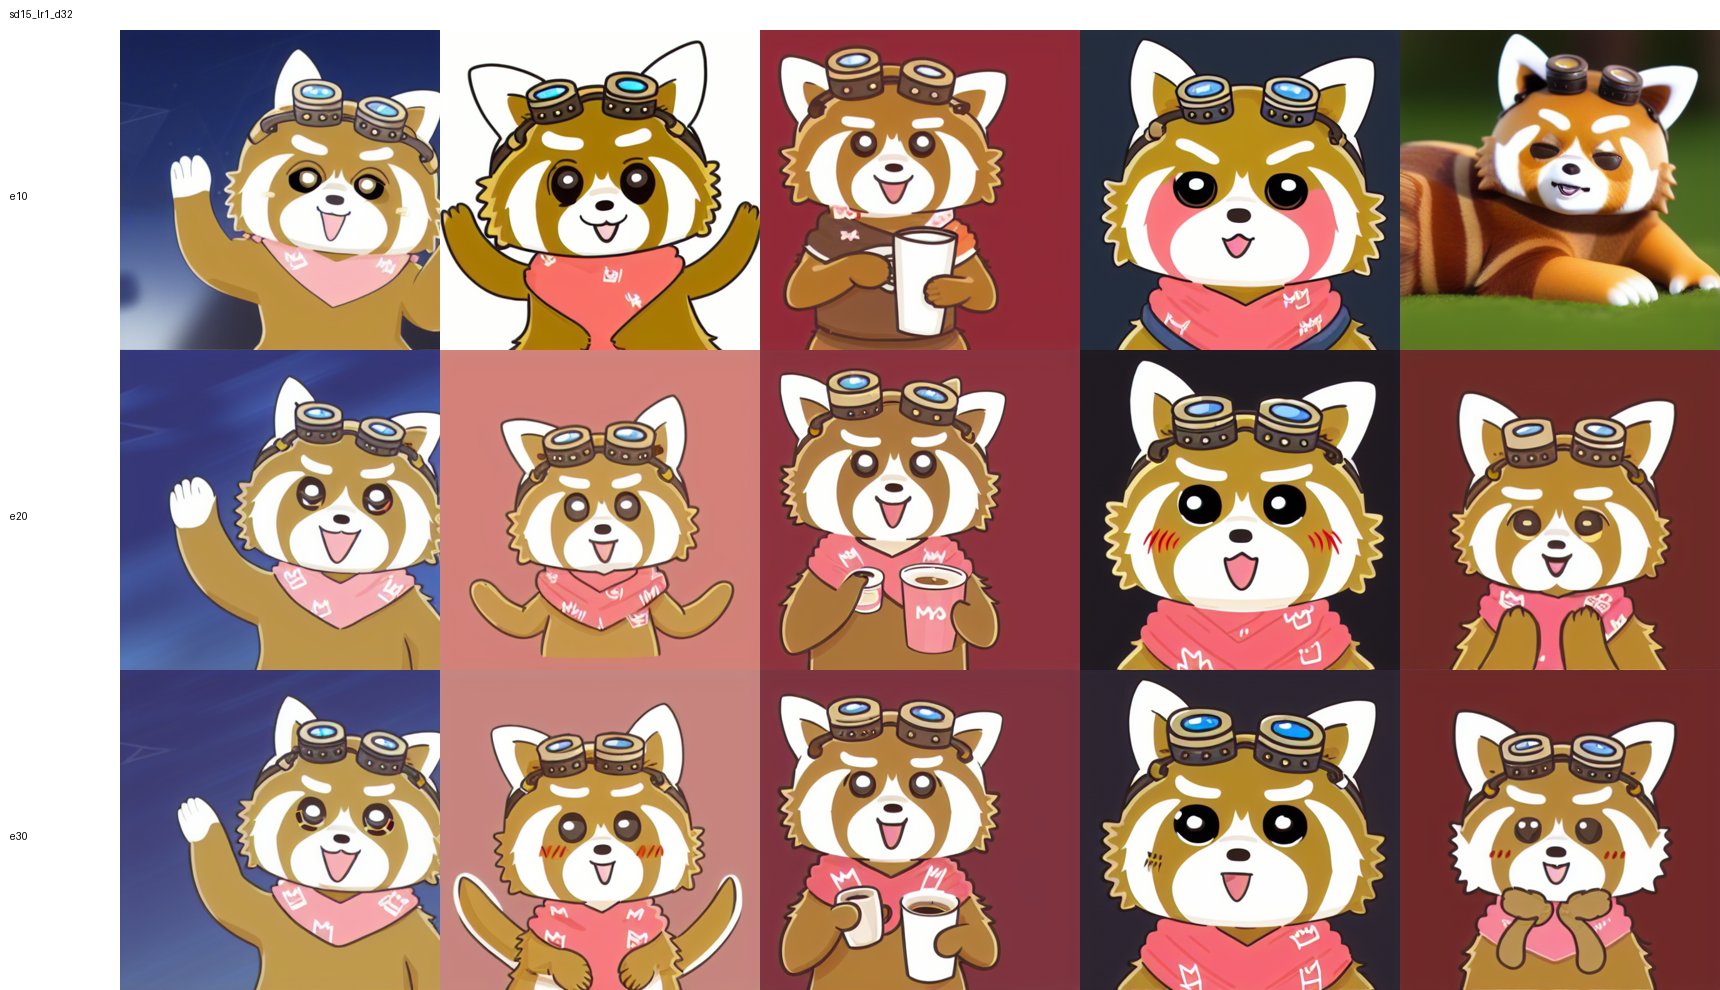
\includegraphics[width=0.78\textwidth]{figures/fig2a_sd15.png}\\[6pt]
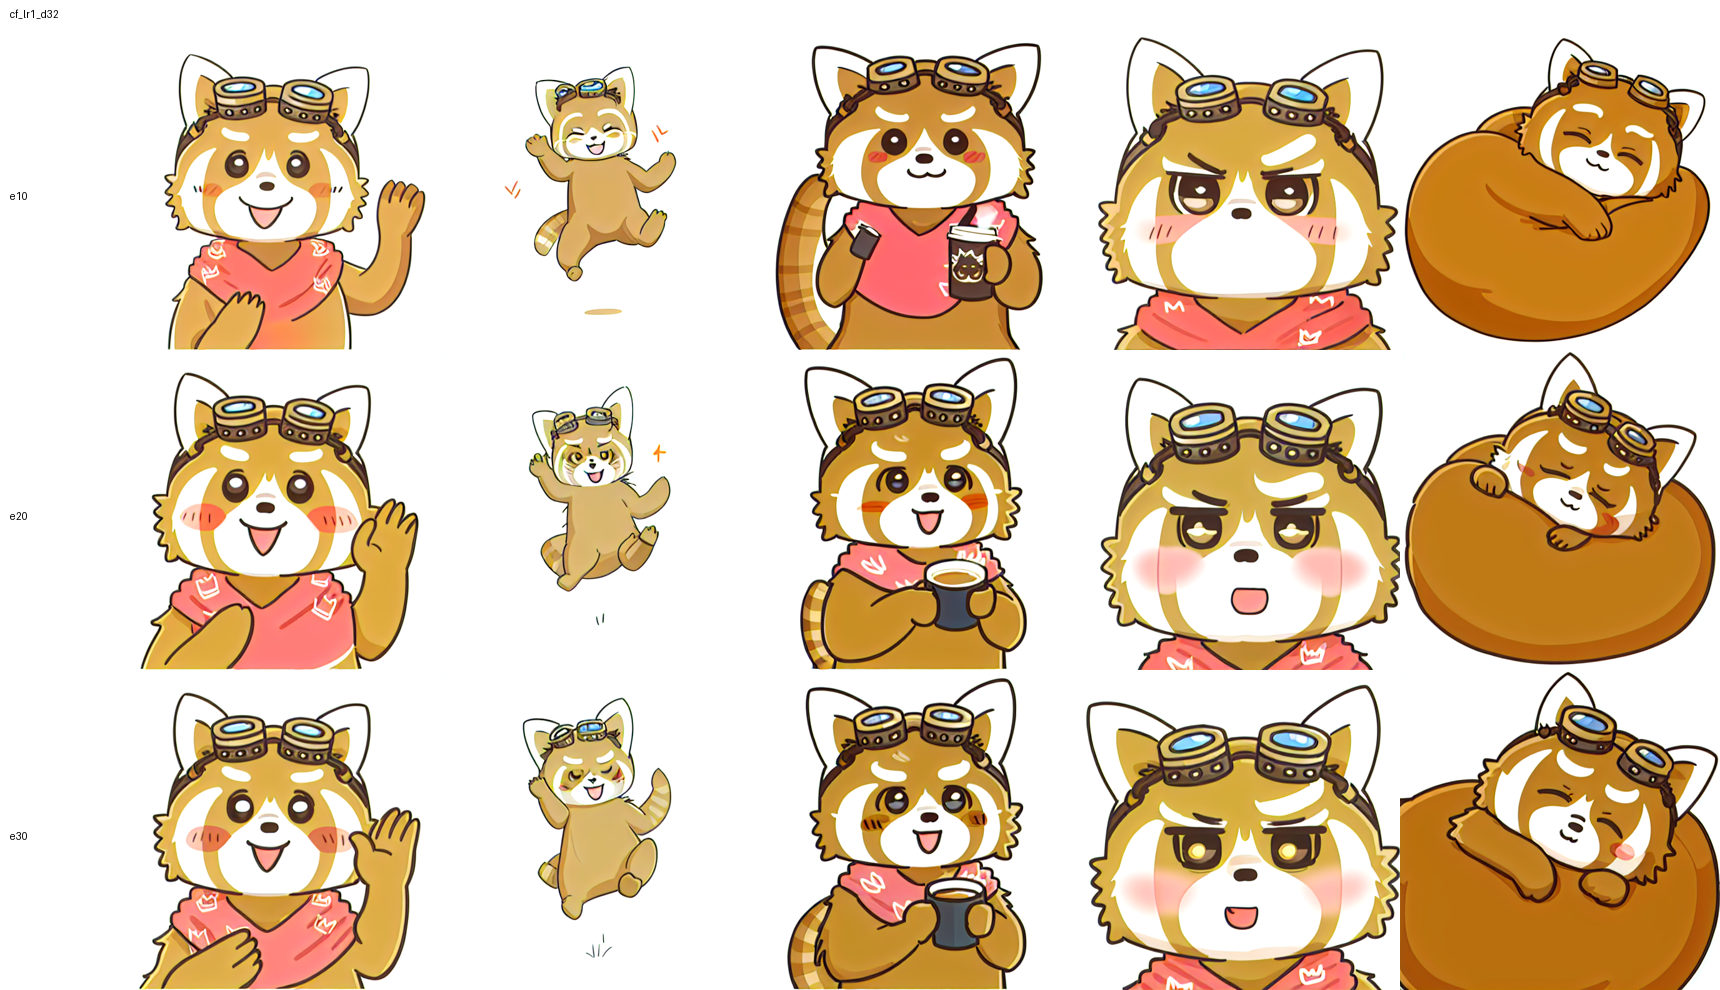
\includegraphics[width=0.78\textwidth]{figures/fig2b_counterfeit.png}
\caption{スイープ比較の代表例。上：標準SD1.5ベース。下：Counterfeitベース。縦軸エポック（10/20/30）、横軸が評価プロンプト。}
\label{fig:sweep}
\end{figure*}

\subsection{実験3：エポック数は約30で頭打ち}
最良条件を60エポックまで延長した結果（図\ref{fig:epoch}）、エポック30/40/50/60の出力はほぼ区別がつかず、\textbf{30エポックの時点で性能はすでに頭打ちに達していた}。エポック50〜60ではむしろ彩度が増し、わずかな過学習の兆候が見られた。\textbf{Q3に対し、本データ・本設定では約30以降は品質が向上しないと結論する。}

\begin{figure*}[t]\centering
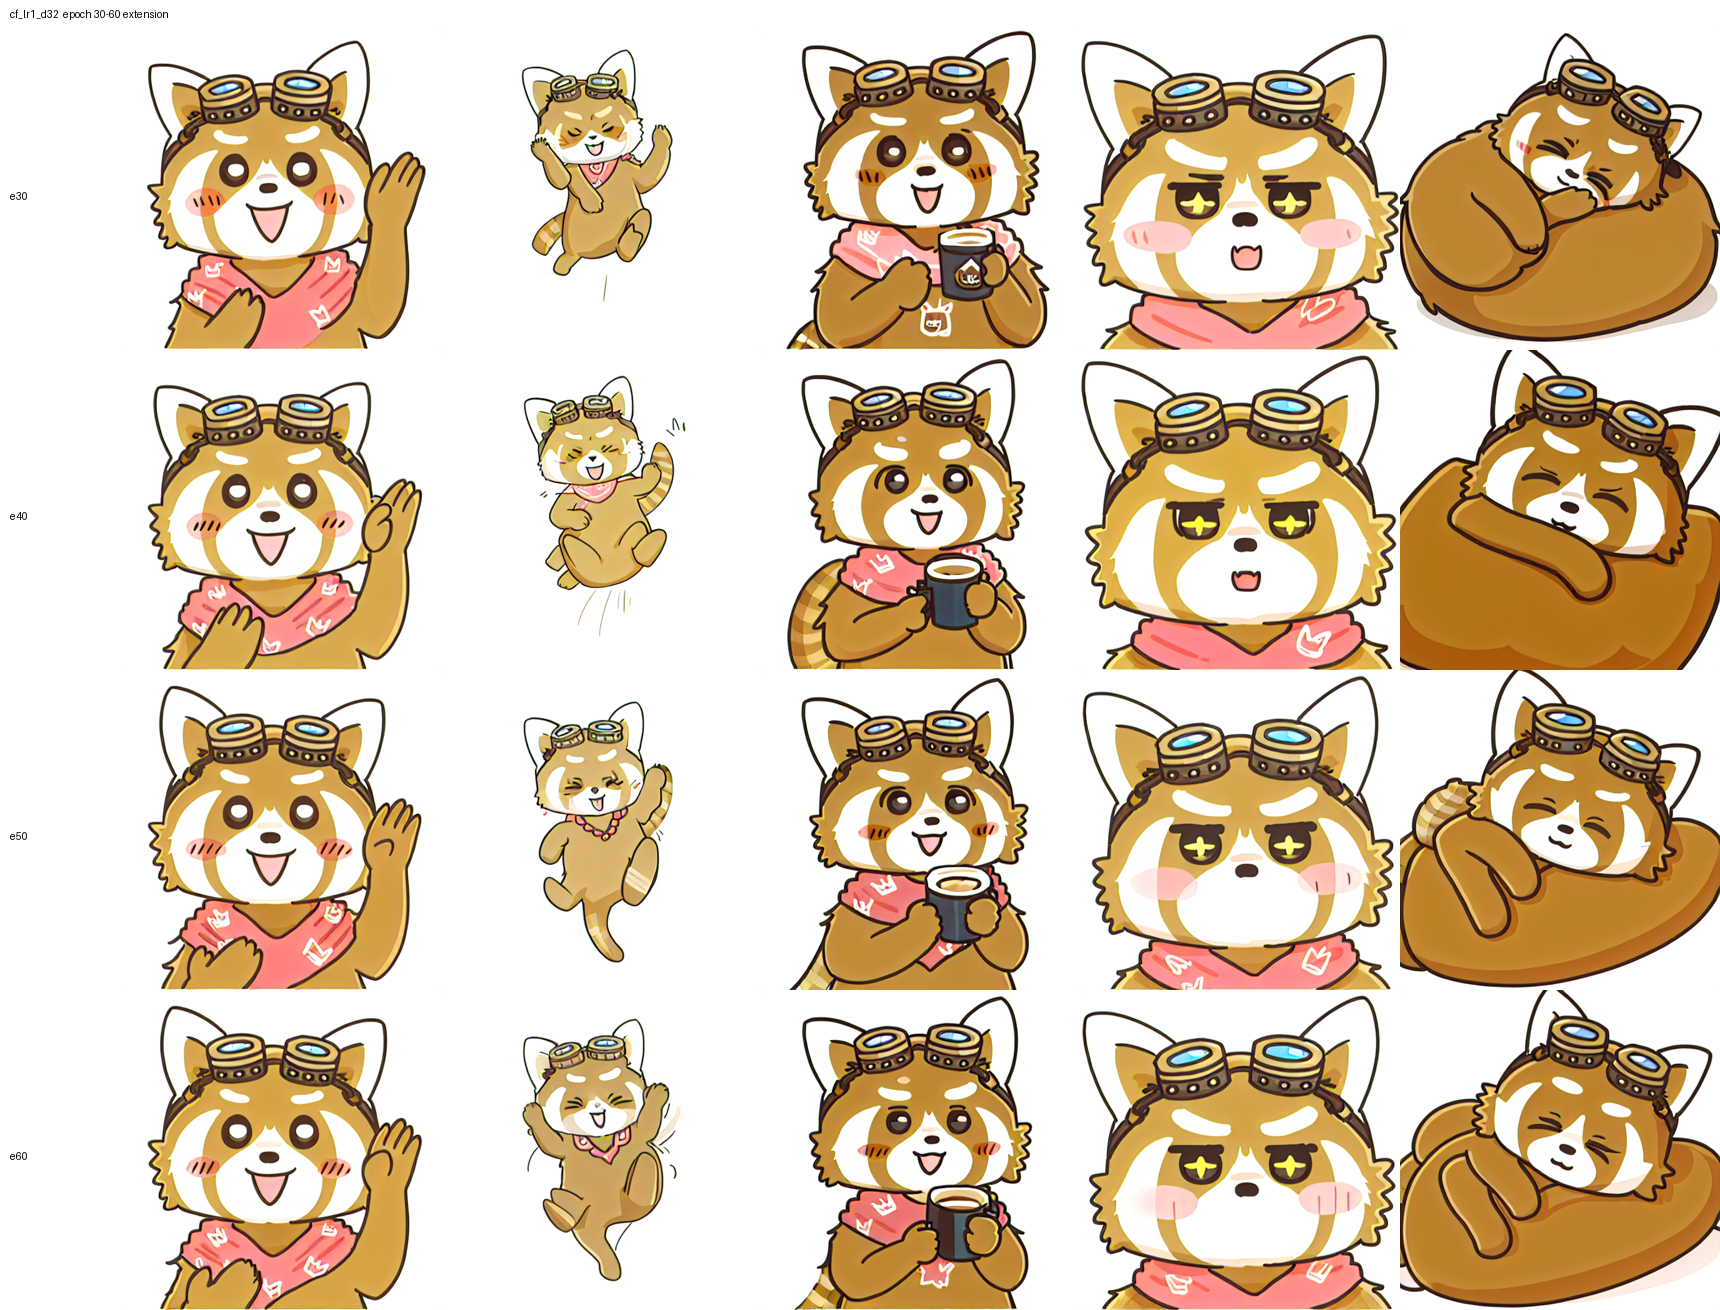
\includegraphics[width=0.78\textwidth]{figures/fig3_epoch.png}
\caption{cf\_lr1\_d32 をエポック30/40/50/60で比較。各行間の差はわずかである。}
\label{fig:epoch}
\end{figure*}

\subsection{最終モデルによる生成}
最良モデル（cf\_lr1\_d32, エポック30）を用いて、学習データに無い12種の場面を生成した（図\ref{fig:showcase}）。いずれもキャラクターの同一性とフラットな画風を保ち、実用に足る品質であった。なお背景の明るさなどシーン依存の属性は、プロンプトに明示的に指定すべきであるという実務的知見も得られた。

\begin{figure*}[t]\centering

\includegraphics[width=0.82\textwidth]{figures/fig4_showcase.png}
\caption{最良モデルによる新規12ポーズの生成例。}
\label{fig:showcase}
\end{figure*}

\section{考察}
\textbf{ベースモデルの支配性。} 出力品質はベースモデルの選択に強く依存する。学習対象の画風（フラットなイラスト）に合ったベースモデルを選ぶことが、ハイパーパラメータ調整よりも優先される。

\textbf{過学習とエポック数。} 13枚という少数データでは約30エポックで学習が飽和する。それ以上の学習は品質を向上させず、過学習のリスクを高める。「長時間学習すれば良くなる」という直感は誤りである。

\textbf{データ量が品質の上限を決める。} エポック数が頭打ちである以上、さらなる品質向上の主たる手段は学習画像の追加である。

\textbf{消費者向けGPUの十分性。} 各学習は RTX 3060 で9〜40分、VRAM使用量は3〜8GBであり、SD1.5 のキャラクターLoRA作成において有料クラウド環境は必須ではない。

\section{限界と今後の課題}
評価は比較グリッドの目視によるもので定量指標を用いていない。学習画像は13枚・対象は1キャラクターであり一般化には限界がある。文字の焼き込みはキャプション記述で対処し、除去の効果は未検証である。今後は学習画像の追加、定量評価指標の導入、SDXL等での検証が課題である。

\section{結論}
著者制作のキャラクター「マサフィー」を対象に、消費者向けGPU（RTX 3060）のみで画像生成LoRAのファインチューニングを行った。13枚の学習画像でキャラクターの同一性を保った新規ポーズ生成が可能であること（Q1）、出力品質はベースモデルの選択に最も強く依存すること（Q2）、約30エポックで性能が頭打ちとなること（Q3）を実証した。本研究は、個人所有キャラクターの追加学習が、有料クラウド資源を用いずとも消費者向けGPU 1台で実用的に完結可能であることを示すものである。

\appendix
\section{主要ハイパーパラメータ（cf\_lr1\_d32）}
ベースモデル: Counterfeit-V3.0／解像度: 768$\times$768／LoRA次元・alpha: 32・16／学習率: 1e-4（cosine）／最適化: 8-bit AdamW／バッチサイズ: 2／エポック数: 30（推奨, 約1950ステップ）／混合精度: bfloat16／データ拡張: 左右反転／注意機構: SDPA。

\end{document}
